\chapter{Upload and manage images}\label{cha:upload-manage-images}

A virtual machine image, referred to in this document simply as an
image, is a single file that contains a virtual disk that has a
bootable operating system installed on it. Images are used to create
virtual machine instances within the cloud.  The image files
themselves are never modified, but you can copy the image into a persistent instance (see chapter \ref{cha:launch-manage-inst}).

As a user of the VSC cloud, you can upload and manage your own virtual
machine images.  For information about creating image files, see the
\href{https://docs.openstack.org/image-guide/}{\emph{OpenStack Virtual
    Machine Image Guide}}.

\strong{Note:} Shared storage in the VSC cloud is connected to a separate network, which is only accessible from within the OpenStack environment.  Therefore, if you want to access your VM from outside of OpenStack, and use the shared storage at the same time, you must make sure your VM image is configured use multiple network interface cards (NICs).

You can choose who can access an image you have created.  The following access policies for images exist:
\begin{description}
\item[public] Public images are provided by the VSC, and can be accessed by all users.
\item[private] If you create a private image, only members of the same
  project have access.
\item[shared] You can also choose to share your image with a list of
  other projects.
\item[community] Community images are user-created images which are
  freely accessible to all other users.
\end{description}

\strong{Note:} You can also use the \textbf{openstack} and
\textbf{glance} command-line clients or the Image service to manage
images.

\subsubsection{Upload an image}
Follow this procedure to upload an image to a project:

\begin{enumerate}
\item Open the Compute tab and click Images category.
\item Click Create Image.

  The Create An Image dialog box appears.
  \begin{center}
    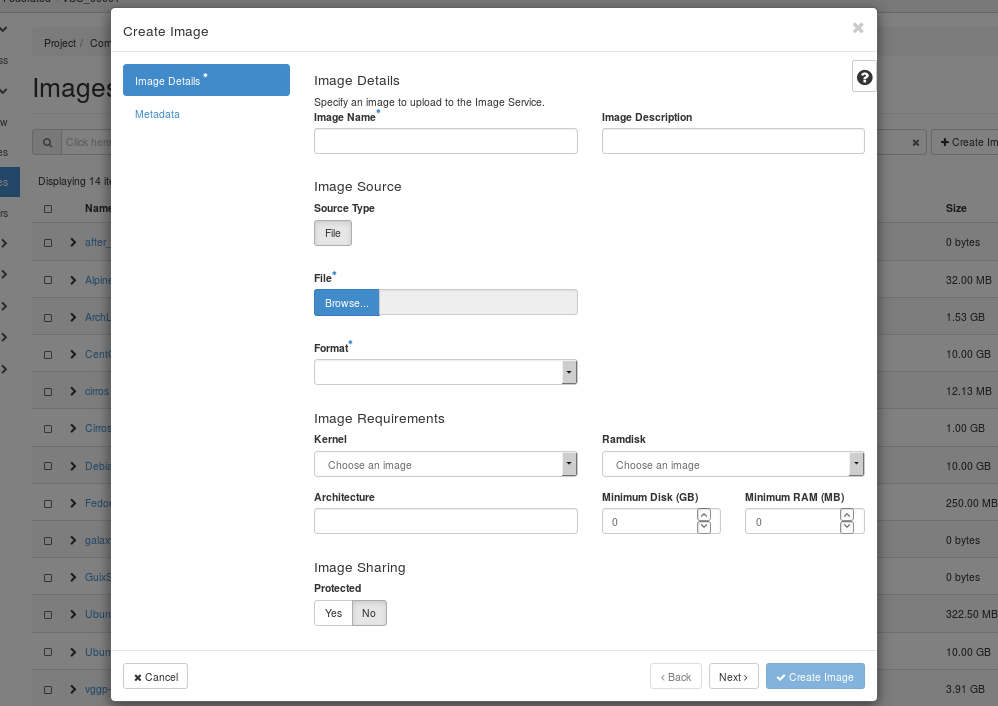
\includegraphics[scale=0.4]{img/tab-compute-images-create.png}
  \end{center}

\item Enter the following values:
  \begin{description}
  \item[Image Name] Enter a name for the image.
  \item[Image Description] Enter a brief description of the image.
  \item[Image Source]\ 
    \begin{description}
    \item[File] Browse for the image file on your file system and add
      it.
    \item[Format] Select the image format (for example, QCOW2) for the
      image.
    \end{description}
  \item[Image Requirements]\ 
    \begin{description}
    \item[Architecture] Specify the architecture. For example,
      \strong{i386} for a 32-bit architecture or \strong{x86\_64} for
      a 64-bit architecture.
    \item[Kernel, Ramdisk] Can be left empty, as this is determined by
      the image file.
    \item[Minimum Disk (GB), Minimum RAM (MB)] Choose suitable values,
      according to the requirements of your image's operating system.
    \end{description}
  \item[Protected] If set to \strong{Yes}, users need to unlock the
    image before they are able to delete it.
  \item[Metadata] You can add resource metadata in this tab. The
    glance Metadata Catalog provides a list of metadata image
    definitions.
  \end{description}
\item Click \strong{Create Image}.
  The image is queued to be uploaded. It might take some time before
  the status changes from Queued to Active.
\end{enumerate}

Another way to create an image is to check-mark on the left side one of the available images and then click on Launch on the right of the screen. That way the mandatory fields in 'Image Details' tab in the 'Create Image' pop-up dialog are automatically filled and the user will be directly presented with the 'Launch Instance'.

\begin{center}
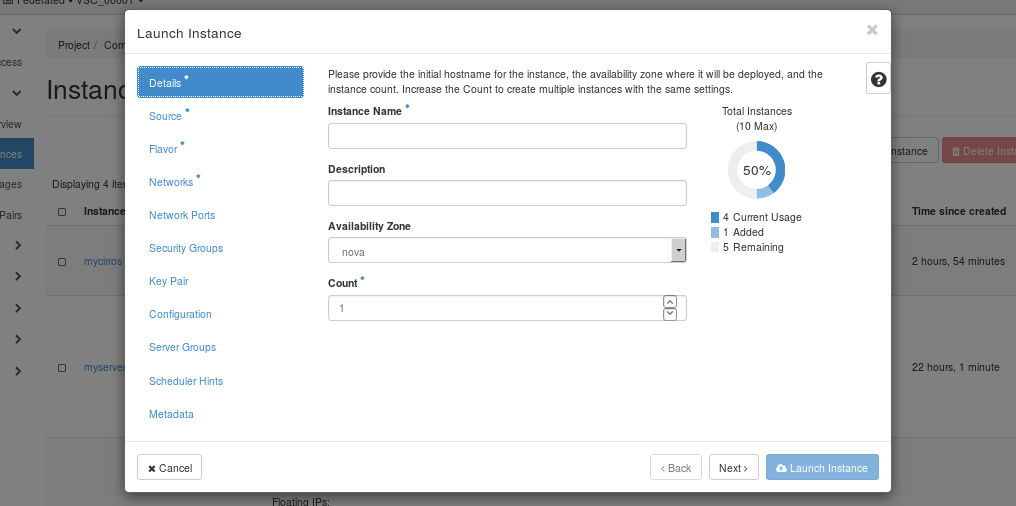
\includegraphics[scale=0.5]{img/tab-compute-instances-launch.png}
\end{center}

\subsubsection{Update an image}

Follow this procedure to update an existing image.

\begin{enumerate}
\item Open the project tab and click the Images category.
\item Select the image that you want to edit.
\item In the Actions column, open the drop-down menu and select
  \strong{Edit Image}.
\item In the Edit Image dialog box, you can perform various
  actions. For example:
  \begin{itemize}
  \item    Change the name of the image.
  \item    Change the description of the image.
  \item    Change the format of the image.
  \item    Change the minimum disk of the image.
  \item    Change the minimum RAM of the image.
  \item    Change the protected status of the image.
  \item    Change the metadata of the image.
  \end{itemize}
\item  Click \strong{Edit Image}.
\end{enumerate}

%%% Local Variables:
%%% mode: latex
%%% TeX-master: "intro-Cloud"
%%% End:
